\subsection{Universal Mobile Telecommunication System (UMTS)}
\label{sub:UMTS}
UMTS se plantea cono una evolución de los sistemas GSM, ya que, los operadores desean proteger su inversión actual. Se plantea un sistema de versiones anuales, desde la primera versión, la Release 99 estable desde marzo del 2000, hasta la actual versión, Release 5, y las futuras, Release 6 y 7. UMTS surge ante la necesidad de: aumentar la capacidad de los servicios básicos de voz y añadir nuevos servicios de datos y multimedia basados en tecnologías de paquetes y protocolos IP. Se pretende ofrecer, 144kbps en entornos rurales, 348kbps en entornos urbanos alcanzando el máximo de 2Mbps en interiores. Otro punto inportante del planteamiento de UMTS es el aumento de la tecnología de roaming y la capacidad de crear terminales reconfigurables, que puedan aumentar sus capacidades mediante la descarga de servicios y aplicaciones.\\
Se crean tres tecnologías que evolucionan de unas a otras:
\begin{itemize}
	\item Global Packet Radio Service (GPRS):permite el acceso radio en modo paquete con backbone IP. Incorpora dos nuevos nodos de conmutación de paquetes al sistema GSM. Permite la transmisión de datos hasta una tasa teórica de 144kbps. Permite la conexión de terminales que utilicen hasta 8 slots para la transmisión.
	\item Enhanced Data rate for Global Evolution (EDGE): Se trata de una evolución del GPRS con modulación y codificación adaptativa. Necesita estaciones base y moviles modificados para utilizar este sistema. A cambio ofrece tasas de transmisión de hasta 384kbps.
	\item EDGE Evolution: Este sistema consigue una gran cuota de mercado al ofrecer tasas de hasta 1Mbps, con modulaciones de hasta 32QAM y utilización de 10 slots de tiempo. Como contra necesita 2 antenas en los terminales y el uso de turbo códigos.
\end{itemize}
\subsubsection{Estándar GPRS}
\label{ssub:GPRS}
	GPRS nace de la necesidad de conectar el sistema GSM directamente a un backbone basado en IP que cada vez se extiende más. Es por esto que GPRS se considera más como un sistema de transición entre los sistemas de segunda generación, GSM, y los de tercera generación, UMTS. Las características principales del sistema GPRS son las siguientes: los datos se encapsulan en mensajes cortos con una cabecera del estilo a la cabecera IP, los recursos de red solo se utilizan cuando hay algo que transmitir, el principal objetivo es el acceso a redes de datos. GPRS reaprovecha las estructuras de GSM añadiendo unicamente dos elementos de red. El nodo GGSN actúa como una pasarela entre la red GPRS y las redes públicas de datos, como la red IP o incluso otras redes GPRS. El nodo SGSN es un servidor dentro de la propia red GSM para dar soporte a la llegada de datos.
\begin{figure}[H]
\centering
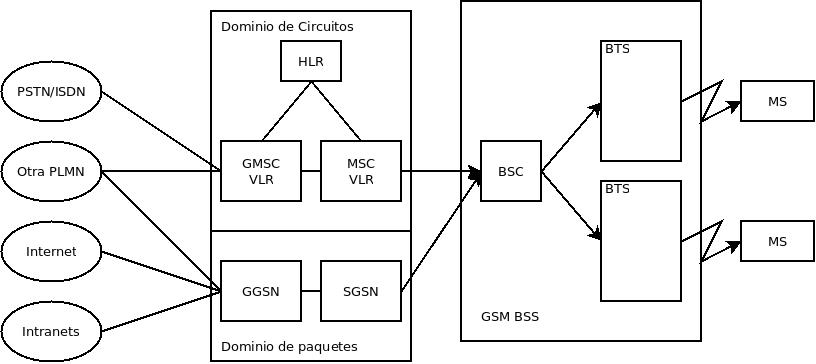
\includegraphics[width=\textwidth]{Imagen/diaGPRS.jpg}
\caption{Estructura de la red GPRS}
\label{img:estructuraGPRS}
\end{figure}
% subsubsection GPRS (end)
\subsubsection{3rd Generation Pertnership Project 3GPP}
\label{ssub:3GPP}
	Consorcio de grupos de estandarización para generar las especificaciones de UMTS. Está formado por grupos de todo el mundo, como el ETSI. 
% subsubsection 3GPP (end)
\subsubsection{UMTS}
\label{ssub:UMTS}
\begin{figure}[H]
\centering
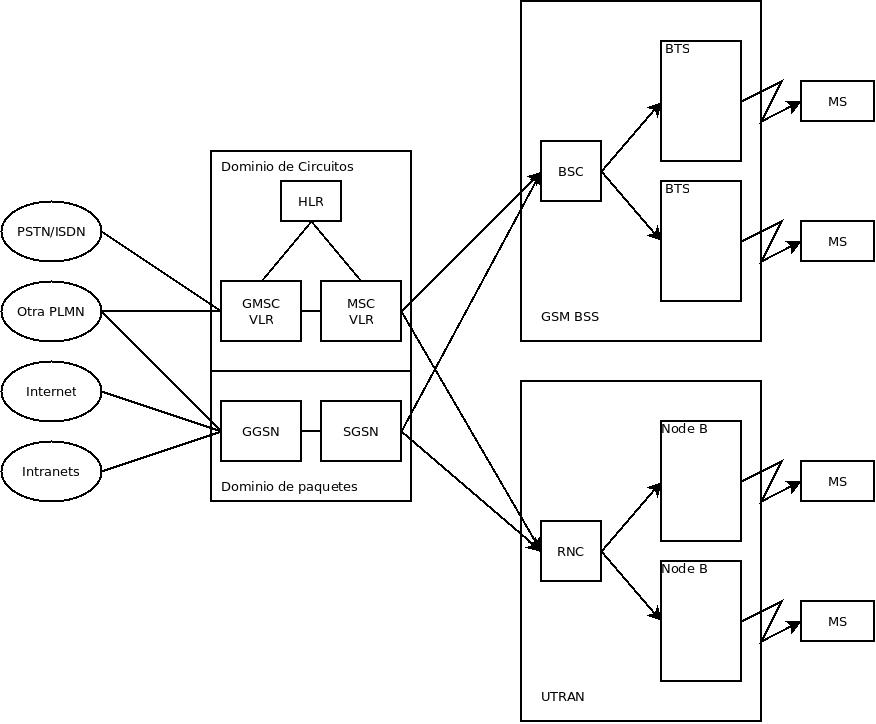
\includegraphics[width=\textwidth]{Imagen/diaUMTS.jpg}
\caption{Estructura de red del sistema UMTS}
\label{img:UMTS}
\end{figure}
La red troncal del sistema UMTS es una evolución de la del sistema GPRS+GSM. Mantiene la separación de los dominios de paquetes y de circuitos aunque presenta una tendencia hacia el dominio único de datos. Se encarga del transporte de la información, tanto del tráfico como de la señalización.\\
La red troncal también tiene toda la intelegincia del sistema, encaminamiento y control y gestión de la movilidad. La red troncal cuenta con los mismos elementos que su antecesora pero se denominan de forma diferente. El HLR, VLR, AuC, EIR y los centros de SMS son los únicos que mantienen su nombre original. Los elementos de ambos dominios MSC, GMSC, SGSN y GGSN pasan a denominarse igual pero con una U delante; U-MSC, U-GMSC, U-SGSN, U-GGSN.\\
La red de acceso tiene una arquitectura similar a la de GSM, pero los elementos se han denominado de forma distinta. Las BTS han pasado a denominarse nodos B y los BSC han pasado a ser Radio Network Controller (RNC). La red de acceso a su vez ha cambiado de ser la BSS a ser la Radio Network System (RNS). Surge también una interfaz entre los RNC que no existía en GSM, que se denomina Iur. El acceso radio cambia de ser un sistema FDD/FDMA/TDMA a utilizar la tecnología CDMA. Esta tecnología utiliza espectro ensanchado para la transmisión de la información, es decir, todos los usuarios de la celda comparten la misma portadora de 5MHz utilizando distintos códigos para distinguir su señal. UMTS utiliza FDD o TDD para la duplexación, dependiendo de si el canal de subida está en otra portadora o en otro slot temporal será una o la otra.
% subsubsection UMTS (end)
\subsubsection{High Speed Downlink Packet Acces (HSDPA)}
\label{ssub:HSDPA}
HSDPA es una mejora de WCDMA para aumentar la tasa binaria del enlace descendente. Permite tasas de transmisión teóricas de hasta 14Mbps, en la práctica existirá una limitación de 10.7Mbps. También permite reducir la latencia de los servicios de datos. Las mejoras técnicas presentadas en esta tecnología son las siguientes: modulación/codificación adaptativas, asignación rápida de recursos y los mecanismos de retransmisión híbridos (HARQ). También se ha introducido una modificación del esquema de gestión de recursos radio, en vez de controlar la potencia de transmisión para mantener la tasa binaria constante. Se utiliza la máxima tasa soportada con la potencia disponible. A lo anterior se suma una nueva técnica de asignación de recursos, asigna los recursos al usuario con mejores condiciones relativas. Esto es mucho mejor cuando las condiciones entre usuarios no están correlacionadas y cuando el número de usuarios es bastante alto, cambiando el usuario con mayor calidad de enlace con mayor facilidad. Otra mejora incluida son los mecanismos de retransmisión híbrida, es decir, en caso de que se produzca una retransmisión no se retransmite todo, si no que se retransmiten solo ciertas partes del paquete, haciendo menor uso de los recursos.\\
Una mejora a este sistema se denomina HSDPA+ o HSPA2. Este nuevo sistema incluye dos portadoras de 5MHzsimultaneas para mejorar la eficiencia espectral y permitir balance de carga entre portadoras.
% subsubsection HSDPA (end)
% subsection UMTS (end)